\documentclass{beamer}
\usepackage{tikz}
\usepackage{hyperref}
\usepackage{listings}
\usepackage{xcolor}

\lstset{
  basicstyle=\ttfamily\small,
  breaklines=true,
  columns=fullflexible,
  frame=single,
  backgroundcolor=\color{gray!10},
  keywordstyle=\color{blue},
  commentstyle=\color{green!50!black},
  stringstyle=\color{red!60!black},
  numberstyle=\tiny,
  numbers=left,
  numbersep=5pt,
  showspaces=false,
  showstringspaces=false,
  captionpos=b
}

\title{Campus Network Design and Implementation}
\subtitle{Computer Network-1 Course Project}
\author{Theodoros}
\institute{Contributors: }
\begin{document}

\begin{frame}
\titlepage
\end{frame}

\begin{frame}
\frametitle{Contents}
\begin{itemize}
    \item \hyperlink{design-diagram}{1. Network Design}
    \item \hyperlink{config}{2. Network Configuration}
    \item \hyperlink{routing}{3. Static/Dynamic Routing}
    \item \hyperlink{dhcp}{4. DHCP Configuration}
    \item \hyperlink{vlans}{5. VLAN Configuration}
    \item \hyperlink{testing}{6. Network Testing}
\end{itemize}
\end{frame}

\section{Network Design}
\begin{frame}[label=design-diagram]
\frametitle{Network Diagram}
\begin{center}
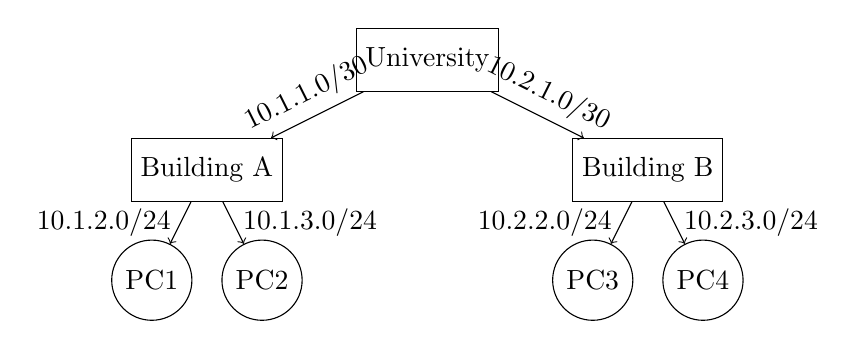
\begin{tikzpicture}[scale=0.7]
    \tikzstyle{router}=[draw, rectangle, minimum width=1.6cm, minimum height=0.8cm]
    \tikzstyle{pc}=[draw, circle, minimum width=0.9cm]
    \node[router] (r1) at (0,0) {University};
    \node[router] (r2) at (-4,-2) {Building A};
    \node[router] (r3) at (4,-2) {Building B};
    \draw[->] (r1) -- node[above,sloped]{10.1.1.0/30} (r2);
    \draw[->] (r1) -- node[above,sloped]{10.2.1.0/30} (r3);
    \node[pc] (pc1) at (-5,-4) {PC1};
    \node[pc] (pc2) at (-3,-4) {PC2};
    \draw[->] (r2) -- node[left]{10.1.2.0/24} (pc1);
    \draw[->] (r2) -- node[right]{10.1.3.0/24} (pc2);
    \node[pc] (pc3) at (3,-4) {PC3};
    \node[pc] (pc4) at (5,-4) {PC4};
    \draw[->] (r3) -- node[left]{10.2.2.0/24} (pc3);
    \draw[->] (r3) -- node[right]{10.2.3.0/24} (pc4);
\end{tikzpicture}
\end{center}
\end{frame}

\section{Network Configuration}
\begin{frame}[label=config]
\frametitle{Network Configuration}
\begin{itemize}
    \item MikroTik RouterOS is used for routers.
    \item Each router uses a unique identity and interface addressing.
    \item PCs have static IP addresses and default gateways.
    \item Subnetting: 10.1.x.x for Building A, 10.2.x.x for Building B.
\end{itemize}
\end{frame}

\begin{frame}[fragile]
\frametitle{Router Configuration: University Router (R1)}
\begin{lstlisting}
system identity set name="university"
ip address add address=10.1.1.1/30 interface=ether1
ip address add address=10.2.1.1/30 interface=ether2
\end{lstlisting}
\begin{itemize}
    \item Connects to Building A and B routers.
    \item /30 subnets for point-to-point links.
\end{itemize}
\end{frame}

\begin{frame}[fragile]
\frametitle{Router Configuration: Building A Router (R2)}
\begin{lstlisting}
system identity set name="Building_A"
ip address add address=10.1.1.2/30 interface=ether1
ip address add address=10.1.2.1/24 interface=ether2 
ip address add address=10.1.3.1/24 interface=ether3
\end{lstlisting}
\begin{itemize}
    \item ether1: Uplink to University Router
    \item ether2: First LAN subnet for PC1
    \item ether3: Second LAN subnet for PC2
\end{itemize}
\end{frame}

\begin{frame}[fragile]
\frametitle{Router Configuration: Building B Router (R3)}
\begin{lstlisting}
system identity set name="Building_B"
ip address add address=10.2.1.2/30 interface=ether1
ip address add address=10.2.2.1/24 interface=ether2    
ip address add address=10.2.3.1/24 interface=ether3
\end{lstlisting}
\begin{itemize}
    \item ether1: Uplink to University Router
    \item ether2: First LAN subnet for PC3
    \item ether3: Second LAN subnet for PC4
\end{itemize}
\end{frame}

\begin{frame}[fragile]
\frametitle{PC Configuration: Building A}
\begin{lstlisting}
# PC1
PC1> ip 10.1.2.2/24 10.1.2.1
# PC2
PC2> ip 10.1.3.2/24 10.1.3.1
\end{lstlisting}
\begin{itemize}
    \item Each PC has a static IP and gateway.
    \item Test: \texttt{ping 10.1.2.1} or \texttt{ping 10.1.3.1}
\end{itemize}
\end{frame}

\begin{frame}[fragile]
\frametitle{PC Configuration: Building B}
\begin{lstlisting}
# PC3
PC3> ip 10.2.2.2/24 10.2.2.1
# PC4
PC4> ip 10.2.3.2/24 10.2.3.1
\end{lstlisting}
\begin{itemize}
    \item Each PC has a static IP and gateway.
    \item Test: \texttt{ping 10.2.2.1} or \texttt{ping 10.2.3.1}
\end{itemize}
\end{frame}

\section{Static/Dynamic Routing}

% University Router RIP
\begin{frame}[fragile,label=routing]
\frametitle{RIP Configuration: University Router}
\begin{lstlisting}
# Enable RIP on relevant interfaces
routing rip interface add interface=ether1 send=v2 receive=v2
routing rip interface add interface=ether2 send=v2 receive=v2
# Tell RIP about directly connected subnets
routing rip network add network=10.1.1.0/30
routing rip network add network=10.2.1.0/30
# Set RIP settings
routing rip set redistribute-connected=yes
routing rip set update-timer=15s
routing rip set timeout-timer=30s
routing rip set garbage-timer=30s
\end{lstlisting}
\end{frame}

% Building A Router RIP
\begin{frame}[fragile]
\frametitle{RIP Configuration: Building A Router}
\begin{lstlisting}
routing rip interface add interface=ether1 send=v2 receive=v2
routing rip interface add interface=ether2 send=v2 receive=v2
routing rip interface add interface=ether3 send=v2 receive=v2
routing rip network add network=10.1.1.0/30
routing rip network add network=10.1.2.0/24
routing rip network add network=10.1.3.0/24
routing rip set redistribute-connected=yes
routing rip set update-timer=15s
routing rip set timeout-timer=30s
routing rip set garbage-timer=30s
\end{lstlisting}


\end{frame}

% Building B Router RIP
\begin{frame}[fragile]
\frametitle{RIP Configuration: Building B Router}
\begin{lstlisting}
routing rip interface add interface=ether1 send=v2 receive=v2
routing rip interface add interface=ether2 send=v2 receive=v2
routing rip interface add interface=ether3 send=v2 receive=v2
routing rip network add network=10.2.1.0/30
routing rip network add network=10.2.2.0/24
routing rip network add network=10.2.3.0/24
routing rip set redistribute-connected=yes
routing rip set update-timer=15s
routing rip set timeout-timer=30s
routing rip set garbage-timer=30s
\end{lstlisting}
\end{frame}

\begin{frame}[fragile]
\frametitle{RIP Command Explanations}
\begin{itemize}
    \item \texttt{routing rip interface add interface=etherX send=v2 receive=v2:} Enables RIP version 2 on the router’s interface. Only interfaces used to connect other routers should run RIP.
    \item \texttt{routing rip network add network=10.X.X.0/YY:} Informs RIP which directly-connected networks to advertise to neighbors.
    \item \texttt{routing rip set redistribute-connected=yes:} Ensures directly-connected networks are included in RIP updates.
    \item \texttt{routing rip set update-timer=15s:} How often RIP sends updates (default = 30s; lower for lab/small network).
    \item \texttt{routing rip set timeout-timer=30s:} If no update is received in 30s, the route is considered invalid.
    \item \texttt{routing rip set garbage-timer=30s:} A route is removed 30s after being marked invalid.
\end{itemize}
\end{frame}

\begin{frame}[fragile]
\frametitle{Verification: End-to-End Connectivity with RIP}
\textbf{Ping from PC3 to PC2 (Building B to Building A):}
\begin{lstlisting}
PC3> ping 10.1.3.2

84 bytes from 10.1.3.2 icmp_seq=1 ttl=61 time=1.491 ms
84 bytes from 10.1.3.2 icmp_seq=2 ttl=61 time=1.291 ms
84 bytes from 10.1.3.2 icmp_seq=3 ttl=61 time=2.439 ms
\end{lstlisting}
\textbf{Ping from PC1 to PC4 (Building A to Building B):}
\begin{lstlisting}
PC1> ping 10.2.3.2

84 bytes from 10.2.3.2 icmp_seq=1 ttl=61 time=1.831 ms
84 bytes from 10.2.3.2 icmp_seq=2 ttl=61 time=1.235 ms
84 bytes from 10.2.3.2 icmp_seq=3 ttl=61 time=2.860 ms
\end{lstlisting}
\textit{Successful replies indicate full network reachability via dynamic routing.}
\end{frame}

\section{DHCP Configuration}
\begin{frame}[fragile,label=dhcp]
\frametitle{DHCP Configuration}
This section will be added later.
\end{frame}

\section{VLAN Configuration}
\begin{frame}[fragile,label=vlans]
\frametitle{VLAN Configuration}
This section will be added later.
\end{frame}

\section{Network Testing}
\begin{frame}[fragile,label=testing]
\frametitle{Network Testing}
This section will be added later.
\end{frame}

\begin{frame}
\frametitle{Conclusion}
\begin{itemize}
    \item \textbf{Current Progress:}
    \begin{itemize}
        \item Network design completed
        \item Basic configuration implemented
        \item Local and routed connectivity established
    \end{itemize}
    \item \textbf{Next Steps:}
    \begin{itemize}
        \item Add DHCP configuration
        \item Add VLAN configuration
        \item Document and test full connectivity
    \end{itemize}
\end{itemize}
\end{frame}

\end{document}